%%%%%%%%%%%%%%%%%%%%%%%%%%%%%%%%%%%%

\section{Data basics}

%%%%%%%%%%%%%%%%%%%%%%%%%%%%%%%%%%%%

\subsection{Observations and variables}

\begin{frame}
\frametitle{Data matrix}

Data collected on students in a statistics class on a variety of variables:

\begin{center}
\begin{tabular}{l cccc l}
		& \hl{variable} \\
		& \hl{$\downarrow$}	 \\
\cline{1-5}
Stu.	&	\var{gender}	&	\var{intro\_extra} & $\cdots$ & \var{dread} \\
\cline{1-5}
1 & male & extravert  & $\cdots$ & 3 \\ 
  2 & female & extravert & $\cdots$ & 2 \\ 
  3 & female & introvert  & $\cdots$ & 4 & \hl{$\leftarrow$}  \\ 
  4 & female & extravert  & $\cdots$ & 2 & \hl{observation} \\
$\vdots$	&	$\vdots$	  &	$\vdots$  &	$\vdots$ &	$\vdots$ \\
86	& male & extravert & $\cdots$& 3 \\
\cline{1-5}
\end{tabular}
\end{center}

\end{frame}

%%%%%%%%%%%%%%%%%%%%%%%%%%%%%%%%%%%%

\subsection{Types of variables}

\begin{frame}
\frametitle{Types of variables}

\begin{center}
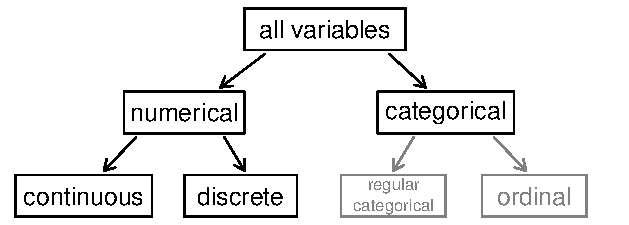
\includegraphics[width=0.9\textwidth]{1-2_data_basics/figures/variables/variables}
\end{center}

\end{frame}

%%%%%%%%%%%%%%%%%%%%%%%%%%%%%%%%%%%

\begin{frame}
\frametitle{Types of variables (cont.)}

\begin{center}
{\footnotesize
\begin{tabular}{c ccc cc}
  \hline
 & \var{gender} & \var{sleep} & \var{bedtime} & \var{countries} & \var{dread} \\
  \hline
1 & male & 5 & 12-2 & 13 & 3 \\ 
  2 & female & 7 & 10-12 & 7 & 2 \\ 
  3 & female & 5.5 & 12-2 & 1 & 4 \\ 
  4 & female & 7 & 12-2 &  & 2 \\ 
  5 & female & 3 & 12-2 & 1 & 3 \\ 
  6 & female & 3 & 12-2 & 9 & 4 \\ 
  \hline
\end{tabular}
}
\end{center}

\begin{itemize}
\item \var{gender}: \pause \soln{\only<2->{categorical}} \pause
\item \var{sleep}: \pause \soln{\only<4->{numerical, continuous}} \pause
\item \var{bedtime}: \pause \soln{\only<6->{categorical, ordinal}} \pause
\item \var{countries}: \pause \soln{\only<8->{numerical, discrete}} \pause
\item \var{dread}: \pause \soln{\only<10->{categorical, ordinal - could also be used as numerical}}
\end{itemize}

\end{frame}

%%%%%%%%%%%%%%%%%%%%%%%%%%%%%%%%%%%

\begin{frame}
\frametitle{Practice}

\pq{What type of variable is a telephone area code?}

\begin{enumerate}[(a)]
\item numerical, continuous
\item numerical, discrete
\solnMult{categorical}
\item categorical, ordinal
\end{enumerate}

\end{frame}

%%%%%%%%%%%%%%%%%%%%%%%%%%%%%%%%%%%

\subsection{Relationships among variables}

%%%%%%%%%%%%%%%%%%%%%%%%%%%%%%%%%%%

\begin{frame}
\frametitle{Relationships among variables}

\dq{Does there appear to be a relationship between number of alcoholic drinks consumed per week and age at first alcohol consumption?}

\begin{center}
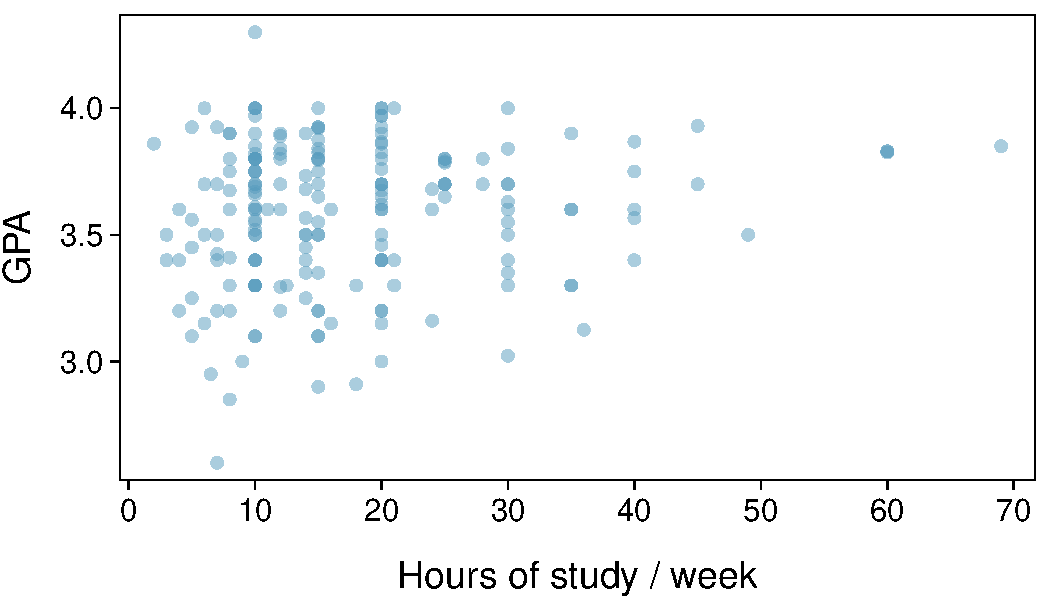
\includegraphics[width=0.7\textwidth]{1-2_data_basics/figures/gpa_study_hours/gpa_study_hours}
\end{center}

\pause

\dq{Can you spot anything unusual about any of the data points?}

\soln{\pause{There is one student with GPA $>$ 4.0, this is likely a data error.}}

\end{frame}

%%%%%%%%%%%%%%%%%%%%%%%%%%%%%%%%%%%

\subsection{Associated and independent variables}

%%%%%%%%%%%%%%%%%%%%%%%%%%%%%%%%%%%

\begin{frame}
\frametitle{Practice}

\twocol{0.5}{0.5}
{
\pq{Based on the scatterplot on the right, which of the following statements is correct about the head and skull lengths of possums?}
}
{
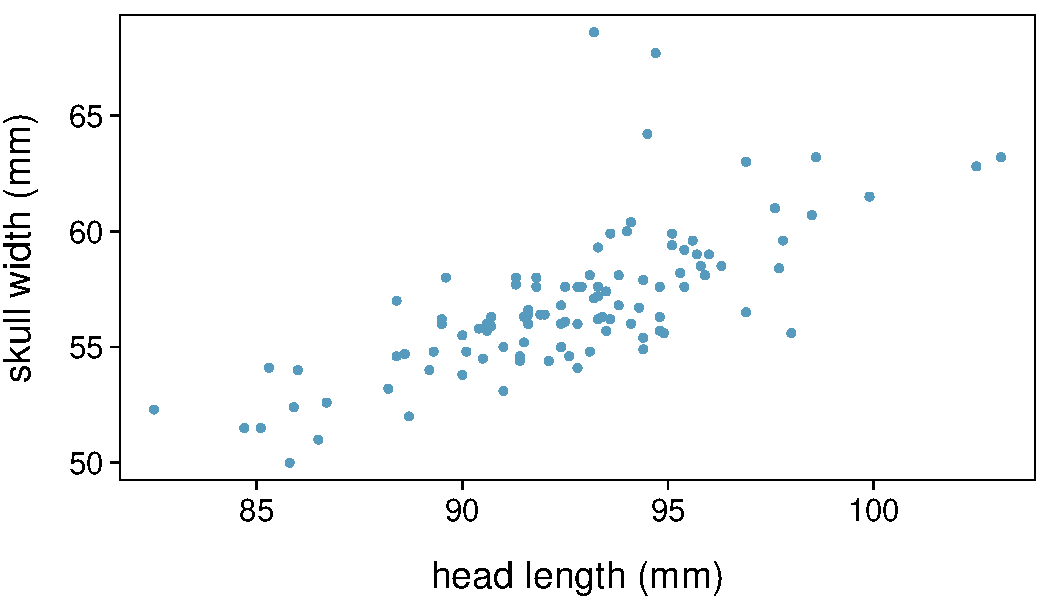
\includegraphics[width=\textwidth]{1-2_data_basics/figures/possum_head_skull/possum_head_skull}
}

\begin{enumerate}[(a)]
\item There is no relationship between head length and skull width, i.e. the variables are independent.
\solnMult{Head length and skull width are positively associated.}
\item Skull width and head length are negatively associated.
\item A longer head causes the skull to be wider.
\item A wider skull causes the head to be longer.
\end{enumerate}

\end{frame}

%%%%%%%%%%%%%%%%%%%%%%%%%%%%%%%%%%%

\begin{frame}
\frametitle{Associated vs. independent}

\begin{itemize}

\item When two variables show some connection with one another, they are called \hl{associated} variables.
\begin{itemize}
\item Associated variables can also be called \hl{dependent} variables and vice-versa.
\end{itemize}

\item If two variables are not associated, i.e. there is no evident connection between the two, then they are said to be \hl{independent}.

\end{itemize}

\end{frame}

%%%%%%%%%%%%%%%%%%%%%%%%%%%%%%%%%%%%